
\begin{document}

\title{AP Calculus AB\&BC}
\author{Hongjun Zeng}
\maketitle

\lipsum[1-10] 

\newpage
\tableofcontents

\newpage
\section{Limits and Continuity}
\subsection{Introducing Calculus}
\newpage
\subsection{Finding Limits Graphically and Numerically}
\subsubsection{An Introduction to Limits}

The limit of a function describes the value that a function approaches as the input approaches some value. Limits are used to define continuity, derivatives, and integrals.

The formal definition of a limit is as follows: 


\begin{Definition}{}{}
Let \( f \) be a function defined on an open interval that contains the point \( c \), except possibly at \( c \) itself. We say that the limit of \( f \) as \( x \) approaches \( c \) is \( L \), and we write:
\[
\lim_{x \to c} f(x) = L
\]
if for every number \( \epsilon > 0 \) there exists a number \( \delta > 0 \) such that if \( 0 < |x - c| < \delta \), then \( |f(x) - L| < \epsilon \).
\end{Definition}

\begin{tcolorbox}[colback=examplebg, colframe=red!75!black, title=\textbf{EXAMPLE 1: Estimating a Limit Numerically}, fonttitle=\bfseries, sharp corners]
\textbf{Evaluate the function} \( f(x) = \frac{x}{\sqrt{x + 1} - 1} \) \textbf{at several \( x \)-values near 0 and use the results to estimate the limit}

\[
\lim_{x \to 0} \frac{x}{\sqrt{x + 1} - 1}
\]


\subsection*{Solution}
The table lists the values of \( f(x) \) for several \( x \)-values near 0.

\textbf{x approaches 0 (left)} \hspace{3cm} \textbf{x approaches 0 (right)}

\begin{tabular}{cccccccc}
\toprule
\( x \)    & -0.01    & -0.001   & -0.0001  & 0     & 0.0001  & 0.001   & 0.01    \\
\midrule
\( f(x) \) & 1.99499  & 1.99950  & 1.99995  & ?     & 2.00005 & 2.00050 & 2.00499 \\
\bottomrule
\end{tabular}
% Using minipage to include the image non-floating
\begin{minipage}{\linewidth}
    \centering
    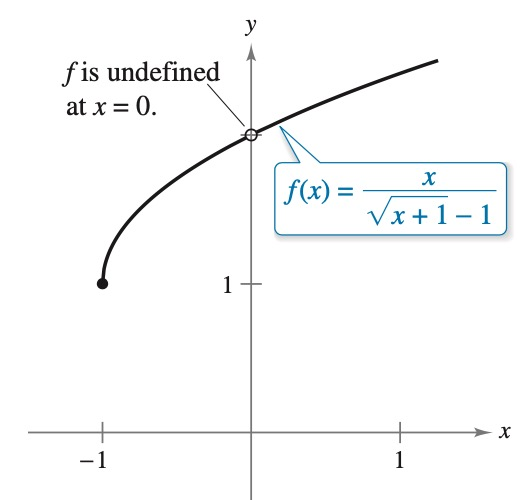
\includegraphics[width=0.37\linewidth]{Example_1.jpg} % Adjust the image width as necessary
    \captionof{figure}{The limit of \( f(x) \) as \( x \) approaches 0 is 2.}
    \label{fig:graph}
\end{minipage}

\end{tcolorbox}

\newpage
\subsubsection{Limits That Fail to Exist}
In calculus, the limit of a function at a certain point is the value that the function approaches as its argument approaches that point. However, not all limits exist. A limit may fail to exist for several reasons, including if the function approaches different values from different directions (left-hand limit and right-hand limit are different), or if the function becomes unbounded near the point, or oscillates indefinitely without settling to a particular value.
\begin{tcolorbox}[colback=examplebg, colframe=red!75!black, title=\textbf{EXAMPLE 2: Different Right and Left Behavior}, fonttitle=\bfseries, sharp corners]

\textbf{Show that the limit
\[
\lim_{x \to 0} \frac{|x|}{x}$
\]
does not exist.}

\subsection*{Solution}
Consider the graph of the function
\[
f(x) = \frac{|x|}{x}.
\]
From the definition of absolute value, we know:
\[
|x| = 
\begin{cases} 
x, & \text{if } x \geq 0, \\
-x, & \text{if } x < 0
\end{cases}
\] % End of absolute value definition

This gives us:
\[
\frac{|x|}{x} = 
\begin{cases} 
1, & \text{if } x > 0, \\
-1, & \text{if } x < 0
\end{cases}
\] % End of function definition

Since the limits as \(x\) approaches zero from the right and left are different, the overall limit does not exist. The function approaches 1 from the right and -1 from the left.
\end{tcolorbox}


\newpage
\subsection{Determining Limits Using Algebraic Properties of Limits}






\subsection{Determining Limits Using Algebraic Manipulation}
\subsection{Selecting Procedures for Determining Limits}
\subsection{Determine Limits Using the Squeeze Theorem}
\subsection{Connecting Multiple Representations of Limits}
\subsection{Exploring Types of Discontinuities}
\subsection{Defining Continuity at a Point}
\subsection{Confirming Continuity over an Interval}
\subsection{Removing Discontinuities}
\subsection{Connecting Infinite Limits and Vertical Asymptotes}
\subsection{Connecting Limits at Infinity and Horizontal Asymptotes}
\subsection{Working with the Intermediate Value Theorem}

\end{document}


\end{document}